\documentclass[UTF8]{article}
\title{插值与数值积分实验报告}
\author{基地班\, \,万宗祺\, \,201600090059}
\date{\today}
\makeatletter
\let\@afterindentfalse\@afterindenttrue
\@afterindenttrue
\makeatother
\setlength{\parindent} {2em}
\usepackage{fontspec}
\renewcommand{\normalsize}{\fontsize{12pt}{\baselineskip}\selectfont}
\usepackage{amsthm}
\usepackage{geometry}
\usepackage[center]{titlesec}
\usepackage{amsfonts}
\usepackage{graphicx}
\usepackage{mathrsfs}
\usepackage{amsmath}
\usepackage{xeCJK}
\usepackage{listings}
\linespread{1.2}
\geometry{left = 2cm,right=2cm,top=2.5cm,bottom=2.5cm}
\begin{document}
\maketitle
\tableofcontents
\section{实验练习10}
\subsection{实验问题}
表1给出的x,y数据位于机翼剖面的轮廓线上,$y_1$和$y_2$分别对应轮廓的上下线.假设需要得到x坐标每改变0.1时的y坐标.试完成加工所需数据,画出曲线,求机翼剖面面积.
\begin{figure}[htbp]
\centering
\textbf{表1.机翼剖面轮廓线数据}

\scalebox{1.1}{
\begin{tabular}{p{0.75cm}|p{0.75cm}|p{0.75cm}|p{0.75cm}|p{0.75cm}|p{0.75cm}|p{0.75cm}|p{0.75cm}|p{0.75cm}|p{0.75cm}|p{0.75cm}}
 \hline
x&0&3&5&7&9&11&12&13&14&15\\
 \hline
y1&0&1.8&2.2&2.7&3.0&3.1&2.9&2.5&2.0&1.6\\
 \hline
y2&0&1.2&1.7&2.0&2.1&2.0&1.8&1.2&1.0&1.6\\
 \hline
\end{tabular}}
\end{figure}
\subsection{实验目的}
(1)熟悉并掌握各种插值方法,并运用到具体问题当中。

(2)掌握用数值积分方法计算复杂平面图形的面积。
\subsection{实验内容}
问题实际上是一个插值问题,为了保证插值的光滑性,我采用了三次样条插值,得到了所需的x坐标每改变0.1时y坐标的数据。最后,我根据得到的数据采用梯形公式来计算出机翼剖面的大致面积,注意在使用trapz函数的时候,要保证图形边界数据点是顺时针顺序给出的。
\subsection{实验求解}
为了解决这个问题,我编写的代码如下:
\lstset{language=Matlab}
\begin{lstlisting}
%ex3_10.m
%%初始数据
x = [0 3 5 7 9 11 12 13 14 15];
y1 = [0 1.8 2.2 2.7 3.0 3.1 2.9 2.5 2.0 1.6];
y2 = [0 1.2 1.7 2.0 2.1 2.0 1.8 1.2 1.0 1.6];
%%三次样条插值
x3 = 0:0.1:15;
y3 = interp1(x,y1,x3,'spline');
y4 = interp1(x,y2,x3,'spline');
%%画图
plot(x3,y3,x3,y4)
%%求面积
S = trapz([x3 x3(end:-1:1)],[y3 y4(end:-1:1)])
\end{lstlisting}
\subsection{实验结果}
运行脚本,得到的机翼轮廓图如下:
\begin{figure}[htbp] 
\centering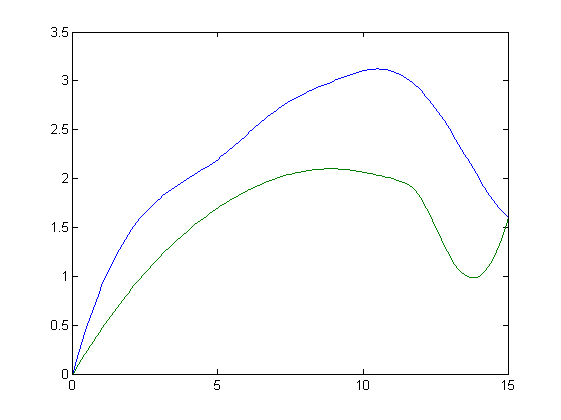
\includegraphics[width=4in]{f1.png} 
\caption{机翼轮廓图}
\end{figure} 

算出的面积S为\textbf{11.3444}
\section{实验练习12}
\subsection{实验问题}
在桥梁的一端每隔一段时间记录1min有几辆车过桥,得到表2的过桥车辆数据:

\begin{figure}[htbp]
\centering
\textbf{表2.过桥车辆数据}

\scalebox{1.1}{
\begin{tabular}{p{1.5cm}|p{1.5cm}||p{1.5cm}|p{1.5cm}||p{1.5cm}|p{1.5cm}}
 \hline
时间&车辆数/辆&时间&车辆数/辆&时间&车辆数/辆\\
 \hline
0:00&2&9:00&12&18:00&22\\
 \hline
2:00&2&10:30&5&19:00&10\\
 \hline
4:00&0&11:30&10&20:00&9\\
\hline
5:00&2&12:30&12&21:00&11\\
\hline
6:00&5&14:00&7&22:00&8\\
\hline
7:00&8&16:00&9&23:00&9\\
\hline
8:00&25&17:00&28&24:00&3\\
\hline
\end{tabular}}
\end{figure}

请估计一天通过桥梁的车流量
\subsection{实验目的}
熟悉并掌握各种插值方法,并运用到具体问题当中。
\subsection{实验内容}
要得到一天内通过得到车流量,需要估计一天中每一分钟的车流量,现在已经给出了一部分的数据,我用样条插值来获得所有的数据。
\subsection{实验求解}
根据题目给出的时间-车辆数数据,构造出分钟-车辆数数据,然后进行插值

练习代码如下:
\lstset{language=Matlab}
\begin{lstlisting}
%ex_12.m
%%初始数据
x = [1 121 241 301 361 421 481 541 631 691 751 841 961 1021 1081 1141 1201 1261 1321 1381 1440];
y = [2 2 0 2 5 8 25 12 5 10 12 7 9 28 22 10 9 11 8 9 3];
%%三次样条插值
x1 = 1:1:1440;
y1 = interp1(x,y,x1,'spline');
%%画图
plot(x1,y1)
%%计算总车流量
total = sum(y1)
\end{lstlisting}
\subsection{实验结果}
运行脚本,得到的时间-车流量图如下:
\begin{figure}[htbp] 
\centering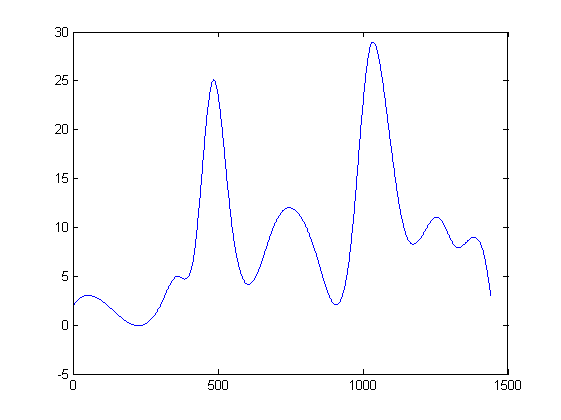
\includegraphics[width=4in]{f2.png} 
\caption{时间-车流量图}
\end{figure} 

最终得到的一天通过车辆数为\textbf{12663}辆

\end{document}